
% Basic template for homeworks
% derived from miktex's article template
% Roger Fowler
% 30 September 2024

\documentclass[10pt]{article} % set font size
\usepackage[utf8]{inputenc} % set input encoding (not needed with XeLaTeX)

\usepackage{geometry} % to change the page dimensions
\geometry{a4paper}

\usepackage{graphicx} % support the \includegraphics command and options
\usepackage{booktabs} % for much better looking tables
\usepackage{array} % for better arrays (eg matrices) in maths
\usepackage{paralist} % very flexible & customisable lists (eg. enumerate/itemize, etc.)
\usepackage{verbatim} % adds environment for commenting out blocks of text & for better verbatim
\usepackage{subfig} % make it possible to include more than one captioned figure/table in a single float
\usepackage{mathtools} % get split environment
\usepackage{amsmath}
\usepackage{cancel} % get /cancel command
\usepackage{tikz} % for drawing geometry
\usepackage{tkz-euclide} % specifically for calculating intersections
\usepackage{amssymb} % get \triangleq
\usepackage{matlab-prettifier} % for including matlab code in a \begin{lstlisting}[style=Matlab-editor] block

\usepackage{fancyhdr} % headers and footers
\pagestyle{plain} % options: empty , plain , fancy

\usepackage{sectsty} % section titles
\renewcommand\thesection{\arabic{section}} % sections are numbered
\renewcommand\thesubsection{\thesection)\alph{subsection}} % subsections are lettered
% options are:
%    \arabic (1, 2, 3, ...)
%    \alph (a, b, c, ...)
%    \Alph (A, B, C, ...)
%    \roman (i, ii, iii, ...)
%    \Roman (I, II, III, ...)
%    \fnsymbol (∗, †, ‡, §, ¶, ...)
%

%\allsectionsfont{\sffamily\mdseries\upshape} % (See the fntguide.pdf for font help)
\usepackage{titlesec}
\titleformat{\section}[hang]
{\normalfont\bfseries}
{\thesection}{0.5em}{}
\titleformat{\subsection}[hang]
{\normalfont\bfseries}
{\thesubsection}{0.5em}{}
\titleformat{\subsubsection}[hang]
{\normalfont\bfseries}
{\thesubsubsection}{0.5em}{}

\renewcommand\deg{^\circ} % define degree symbol as \deg

% matrix display commands
\newcommand{\skewmat}[3]{\begin{bmatrix}0&-#3&#2\\#3&0&-#1\\-#2&#1&0\end{bmatrix}}
\newcommand{\diagmat}[3]{\begin{bmatrix}#1&0&0\\0&#2&0\\0&0&#3\end{bmatrix}}
\newcommand{\vecmat}[3]{\begin{bmatrix}#1\\#2\\#3\end{bmatrix}}

% laplace transform commands
\newcommand{\Lapl}[1]{\mathcal{L}\left\{#1\right\}}
\newcommand{\invLapl}[1]{\mathcal{L}^{-1}\left\{#1\right\}}

% neural network package
%\usepackage{neuralnetwork}

% tikz ellipse
\usetikzlibrary{shapes.geometric}

% rotated text
\usepackage{rotating}

% table stuff
%\usepackage{multicolumn}
\usepackage{multirow}
%\usepackage{tabularx}

%%% END Article customizations

\title{\vspace{-2cm}CS 5180 - Final Project Notes}
\author{Roger Fowler}
\date{MONTH DAY YEAR}

\begin{document}
\maketitle

BIG CHANGES:

switched to pettingzoo because gymnasium is not well set up to handle multiple agents
switched to deep w leaning because state space proved to be infeasibly large

\section{State Definitions}

At the beginning of a hand, a player is dealt a number of cards. It then bets a certain number of tricks between 0 and the number of available tricks, inclusive. When a player is presented with a choice of card to play, there are a number of pieces of information they have:

\begin{enumerate}
\item Cards in their hand
\item Trump suit
\item Led suit
\item Cards which have been played
\item Who led the hand
\item Bet amount
\item Tricks won
\item Tricks remaining
\end{enumerate}

Some of these are simply redundant; who led the hand is obvious by the number of cards in the current trick pile, and is important for the unpredictability of later players. The led suit is also obvious because it is the suit of the first card in the trick pile, and is not defined if there is no pile. Tricks remaining is equal to the number of cards in hand.

Bet amount and tricks won can be combined into the number of tricks that must still be won to make the bet. In this case the agent can only decrease this number and will aim for zero. But decreasing it past zero will incur a penalty at scoring time.

A naive treatment of knowledge about specific cards would produce a massive state space. The 60 card deck is distributed among several groups; with some number of known cards in hand, a known card flipped to reveal trump suit, known cards that have been played, and the rest of the unknown cards distributed between the remaining undealt deck and the other players’ hands. In fact, there is additional information here; a player may not know which specific cards are in another player’s hand, but because a player can be forced to play the led suit, if they do not do so implies that they have no cards of that suit.

Ultimately the game allows for much simplification. Suits are fungible, except that one is the trump suit for the hand and one (possibly the same) is the led suit for the trick. Additionally, cards themselves are fungible. If a player has a set of cards in their hand of a single suit, and knows that there are no cards in other players’ hands of the same suit and between the ranks of the set, then they are all functionally the same card because they have the same chance of winning in a particular situation. Once card values have merged in this way they will never unmerge.

For any game state, since the player knows much about which cards are where or are likely to be where, a card-counting agent can calculate exactly how many cards could appear that would beat a given card. It can then abstract the large amount of information it has into a value for each card, and to combine those cards into groups of cards with the same value. Ultimately, this leads to a representation of the state which is much simplified compared to all of the information the agent actually has. An agent's hidden state is composed of all of the information about exact cards and where they can be. But the agent only needs to know, in the moment, a simplified representation of its hand and how many tricks it must win in the remaining hand, and it will use this simplified state to evaluate its value function. TODO THIS IS UNCLEAR

State transitions become simplified in this representation. A state is composed of a hand of N cards and a goal of T remaining tricks to win. After an action is taken, the rest of the agents take their actions, and the agent arrives at a new state. This state will have exactly N-1 cards, and the agent is in control of which card was removed. However, it is generally not in control of whether T has remained the same or decreased by exactly one. Eventually this leads to a state where there are no cards in hand. In these states, any action (which can be restricted to a single null action) gives a reward and leads to a final terminal state. This reward is only positive when the bet was achieved (T=0) and increasingly negative otherwise. Also, since the agent has no control over the length of the game it does not make sense to discount rewards.

%\def\layersep{2.5cm}
%\begin{figure}[h!]
%\centering
%\begin{tikzpicture}[shorten >=1pt,->,draw=black!50, node distance=\layersep]
%    \tikzstyle{every pin edge}=[<-,shorten <=1pt]
%    \tikzstyle{neuron}=[circle,fill=black!25,minimum size=17pt,inner sep=0pt]
%    \tikzstyle{input neuron}=[neuron, fill=green!50];
%    \tikzstyle{output neuron}=[neuron, fill=red!50];
%    \tikzstyle{hidden neuron}=[neuron, fill=blue!50];
%    \tikzstyle{annot} = [text width=4em, text centered]
%
%    % Draw the input layer nodes
%    \foreach \name / \y in {1,...,4}
%    % This is the same as writing \foreach \name / \y in {1/1,2/2,3/3,4/4}
%        \node[input neuron, pin=left:Input \#\y] (I-\name) at (0,-\y) {};
%
%    % Draw the hidden layer nodes
%    \foreach \name / \y in {1,...,5}
%        \path[yshift=0.5cm]
%            node[hidden neuron] (H-\name) at (\layersep,-\y cm) {};
%
%    % Draw the output layer node
%    \node[output neuron,pin={[pin edge={->}]right:Output}, right of=H-3] (O) {};
%
%    % Connect every node in the input layer with every node in the
%    % hidden layer.
%    \foreach \source in {1,...,4}
%        \foreach \dest in {1,...,5}
%            \path (I-\source) edge (H-\dest);
%
%    % Connect every node in the hidden layer with the output layer
%    \foreach \source in {1,...,5}
%        \path (H-\source) edge (O);
%
%    % Annotate the layers
%    \node[annot,above of=H-1, node distance=1cm] (hl) {Trick 1};
%    \node[annot,left of=hl] {End-Of-Hand States};
%    \node[annot,right of=hl] {Terminal State};
%\end{tikzpicture}
%\caption{State Diagram for an Agent during a Hand}
%\label{fig:states}
%\end{figure}

%\begin{figure}[h!]
%\centering
%\begin{neuralnetwork}
%\newcommand{\h}[2]{$\begin{matrix}\{H(#1)\}\\T=#2\end{matrix}$}
%\newcommand{\p}[4] {$p_{#2,#4}$}
%\setdefaultlinklabel{\p}
%\inputlayer[count=1, bias=false, text=\h]
%\foreach \col in {2,...,4}{ \inputlayer[count=\col, bias=false, text=\h] \linklayers }
%%\foreach \n in {1,...,3}{
%%    \foreach \m in {1,2}{
%%        \link[style={}, labelpos=near start, from layer=0, from node=\n, to layer=1, to node=\m]
%%    }
%%}
%\outputlayer[count=1, text=$S_t$] \linklayers
%\end{neuralnetwork}
%\caption{State Diagram for an Agent during a Hand}
%\label{fig:states}
%\end{figure}

%\begin{figure}[h!]
%\centering
%\begin{tikzpicture}[node distance={15mm}, thick, main/.style = {draw, circle}] 
%%\node[main] (1) {$x_1$};
%%\foreach \row in {2,...,4}{
%%	\node[main] (\row) [right of = \pgfmathsetmacro{\result{\row-1}}] {$a$};
%%%	\foreach \col in {2,...,\row}{
%%%		\node[main] (1) [above right of 
%%%	}
%%}
%%\node[main] (2) [above right of=1] {$x_2$};
%%\node[main] (3) [below right of=1] {$x_3$}; 
%%\node[main] (4) [above right of=3] {$x_4$}; 
%%\node[main] (5) [above right of=4] {$x_5$}; 
%%\node[main] (6) [below right of=4] {$x_6$}; 
%%\draw[->] (1) -- (2); 
%%\draw[->] (1) -- (3); 
%%\draw (1) to [out=135,in=90,looseness=1.5] (5); 
%%\draw (1) to [out=180,in=270,looseness=5] (1); 
%%\draw (2) -- (4); 
%%\draw (3) -- (4); 
%%\draw (5) -- (4); 
%%\draw[->] (5) to [out=315, in=315, looseness=2.5] (3); 
%%\draw[->] (6) -- node[midway, above right, sloped, pos=1] {+1} (4); 
%\node \foreach \col in {1,...,4} \foreach \row in {1,...,\col} [draw] at (\col,\row) {\col,\row};
%\end{tikzpicture} 
%\caption{State Diagram for an Agent during a Hand}
%\label{fig:states}
%\end{figure}

\begin{figure}[h!]
\centering
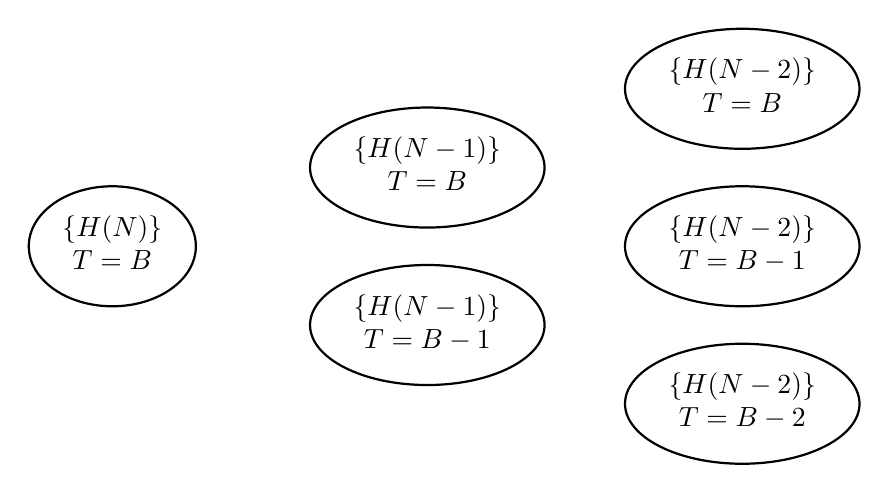
\begin{tikzpicture} [thick, main/.style = {draw,ellipse}]
\def\xsep{2}
\def\ysep{1}
\def\ncols{3}
\newcommand{\nodelabel}[2]{$\begin{matrix}\{H(#1)\}\\T=#2\end{matrix}$}
\node[main] (1) at (\xsep,0) {\nodelabel{N}{B}};
\foreach \i in {2,...,\ncols} {
	\pgfmathtruncatemacro{\in}{1-\i}
	\node[main] (\i*\ncols) at (2*\xsep*\i-\xsep,-2*\ysep+\ysep*\i+\ysep) {\nodelabel{N\in}{B}};
	\foreach \j in {2,...,\i} {
		\pgfmathtruncatemacro{\jn}{1-\j}
		\node[main] (\i*\ncols+\j-1) at (2*\xsep*\i-\xsep,-2*\ysep*\j+\ysep*\i+\ysep) {\nodelabel{N\in}{B\jn}};
	}
}
\end{tikzpicture}
\caption{State Diagram for an Agent during a Hand}
\label{fig:states}
\end{figure}

\subsection{final state representation}

T, sum(T), hand, pile, whether there is a trump suit (because first suit in hand is always trump suit), whether the led suit is the trump suit (as otherwise it would be the second suit, and the case where there is no led suit should be obvious from the pile)

padding this vector with -1 so it is always the same length is good for consistent indexing and convolution

possible hand representations:

\begin{itemize}
\item list of card indices - no consistent convolution-friendly stuff, but this is the format that the env should give as an observation
\item binary list of whether card is in hand
\item binary list of whether card is in hand, sorted by wizard-trump-led-other1-other2-jester suit
\item binary list of whether card is in hand, sorted, with -1 for cards that have appeared - includes info about game state beyond your own hand
\item list of card values evaluated by full card counting
\end{itemize}

Therefore:

\begin{itemize}
\item T
\item sum(T) across players
\item number of players
\item trump suit flag
\item led suit = trump suit flag
\item card state (padded, sorted) =
$\begin{cases}
2 & \text{in pile} \\
1 & \text{in hand} \\
0 & \text{unseen} \\
-1 & \text{in previous piles} \\
\end{cases}$
\end{itemize}

\section{Action Definitions}

The action space is large, but the permissible actions in any given state are small. However many groups of cards are in an agent’s hand are the number of actions available to it.

actions:

\begin{table}[h!]
\centering
\begin{tabular}{|c|c|} \hline
Index & Action \\ \hline
[0, 59] & place card at index $i$ \\ \hline
[60, 80] & bet $i-60$ \\ \hline
[81, 84] & choose suit for trump \\ \hline
[85] & null action used for receiving reward \\ \hline
\end{tabular}
\caption{Action Space Definition}
\end{table}

\section{State Transition}

Starting with the trick leader we proceed around the table comparing cards. If a card is better than the current winner, that card becomes the winner. The possibilities are encoded in Table \ref{tab:trickwinner}.

\begin{table}[h!]
\centering
\begin{tabular}{ccc}
\begin{tabular}{c|l}
\multicolumn{2}{c}{Legend} \\ \hline
Y & New Card Wins \\
X & Current Winner Remains \\
$>$ & Compare Card Values \\
N/A & Impossible \\
\end{tabular}
& \hspace{5mm} &
\begin{tabular}{rrccccc}
\multicolumn{1}{l}{}      & \multicolumn{1}{l}{}        & \multicolumn{5}{c}{Current Winner}                                                                                                                                               \\
\multicolumn{1}{l}{}      & \multicolumn{1}{l}{}        & Wizard                              & Trump                               & Led                                 & Other                    & Jester                              \\ \cline{3-7} 
\multirow{5}{*}{\begin{turn}{90}New Card\end{turn}} & \multicolumn{1}{r|}{Wizard} & \multicolumn{1}{c|}{\textgreater{}} & \multicolumn{1}{c|}{\textgreater{}} & \multicolumn{1}{c|}{\textgreater{}} & \multicolumn{1}{c|}{N/A} & \multicolumn{1}{c|}{\textgreater{}} \\ \cline{3-7} 
                          & \multicolumn{1}{r|}{Trump}  & \multicolumn{1}{c|}{\textgreater{}} & \multicolumn{1}{c|}{\textgreater{}} & \multicolumn{1}{c|}{Y}              & \multicolumn{1}{c|}{N/A} & \multicolumn{1}{c|}{\textgreater{}} \\ \cline{3-7} 
                          & \multicolumn{1}{r|}{Led}    & \multicolumn{1}{c|}{\textgreater{}} & \multicolumn{1}{c|}{X}              & \multicolumn{1}{c|}{\textgreater{}} & \multicolumn{1}{c|}{N/A} & \multicolumn{1}{c|}{\textgreater{}} \\ \cline{3-7} 
                          & \multicolumn{1}{r|}{Other}  & \multicolumn{1}{c|}{\textgreater{}} & \multicolumn{1}{c|}{X}              & \multicolumn{1}{c|}{X}              & \multicolumn{1}{c|}{N/A} & \multicolumn{1}{c|}{\textgreater{}} \\ \cline{3-7} 
                          & \multicolumn{1}{r|}{Jester} & \multicolumn{1}{c|}{\textgreater{}} & \multicolumn{1}{c|}{\textgreater{}} & \multicolumn{1}{c|}{\textgreater{}} & \multicolumn{1}{c|}{N/A} & \multicolumn{1}{c|}{\textgreater{}} \\ \cline{3-7} 
\end{tabular}
\end{tabular}
\caption{Trick Winner Logic}
\label{tab:trickwinner}
\end{table}

\section{Training Procedure}

Hands are independent of one another. The deck is shuffled between hands, so there is no connection in state, and total score is simply a sum of score from each hand. This allows a hand to be played in isolation without having to consider the rest of the game.

Because rewards only occur at the end of a hand, it is reasonable to start training closest to the reward. That is, starting with a hand with a low number of tricks is easier to learn. This also reduces the number of actions an agent can take in each trick, because it has fewer cards in hand. The last tricks of a large hand are similar but not exactly the same as the tricks in a small hand, because the possible number of bet tricks may be very high, and also because the agent has much more knowledge of what has and has not been played. Still, the knowledge should be generalizable, so short hands should be trained before long hands.

Once the agent is able to play for an arbitrary choice of hand and bet, it should be possible to train the agent to choose its own bet as well. These special actions are reserved for only this phase of play. In reality since this stage of play is completely divorced this choice could be handed off to a different specialized agent, except that this agent would need access to the expected rewards of starting each hand with a given bet. Actions are already restricted by play, so it is not a serious complication to have special actions reserved for only this situation. This also does not require any additional state information.

There is one more special state; the dealer turns over the top card of the deck to set the trump suit after dealing the hand. If this card is a Wizard, the dealer is able to choose the trump suit. Again, this creates four actions that only occur in this rare situation. And again, access to the state value function is useful to train this, and no additional state information is necessary, so it can be rolled into the larger agent. Since this choice appears before the choice of bet and before play, it should be trained last. During training this choice should be taken randomly.

\end{document}
